\documentclass[conference]{IEEEtran}
\usepackage{cite}
\usepackage{amsmath,amssymb}
\usepackage{graphicx}
\usepackage{booktabs}
\usepackage{multirow}
\usepackage{url}
\usepackage[caption=false,font=footnotesize]{subfig}

\newcommand{\dd}{Defective Damper}
\newcommand{\map}{mAP@0.5}

\begin{document}

\title{Data-Centric Rare-Defect Detection for Autonomous Transmission-Line Inspection with Nano-Scale Detectors}

\author{
\IEEEauthorblockN{Author List Pending\thanks{Working draft --- author list, contact details, and funding statement to be finalized before submission.}}
\IEEEauthorblockA{Department of Electrical and Computer Engineering\\
University of Nevada, Las Vegas\\
Las Vegas, NV, USA}
}

\maketitle

\begin{abstract}
Uncrewed-aerial-vehicle (UAV) inspection of overhead transmission lines with deep object detectors is limited by scarce annotated defect data, most acutely for \emph{rare} defect classes: in the ATLI benchmark, the Defective Damper class provides 113 instances against 1{,}460 Normal Dampers and is among the weakest classes for the originating transfer-learning baselines, mirroring damper results across the field. This paper reports a systematic, data-centric study of that bottleneck. Harvesting external data does not fix it: community damper datasets at every mixing dose, scale-matched curation, staged pretraining, and in-domain source pretraining all fail to improve the rare class---a label-style and domain mismatch expressed as a recall drop. A \emph{native-only} recipe---1280\,px training, $3\times$ oversampling of damper-bearing images, and scale-down augmentation---raises YOLOv11n from 0.722 to 0.785 \map{} and from 0.743 to 0.812 Defective Damper AP under proper 5-fold cross-validation, matching a 47M-parameter DINO-4scale on mAP and remaining comparable on the rare class (paired per-fold $\Delta{=}{+}0.023\pm0.050$) at ${\sim}18\times$ fewer parameters. A perceptual-hash provenance audit exposes evaluation-set contamination from three public datasets; the recipe's margin survives decontamination. A 768\,px retrain exports to a Jetson-Nano-targeted TensorRT FP16 engine at a cost of 0.009 \map{}; on-device throughput is projected, not yet measured. On small inspection datasets, disciplined evaluation and native data-centric training beat both external data harvesting and parameter-heavy architectures.
\end{abstract}

\begin{IEEEkeywords}
transmission line inspection, defect detection, UAV, transfer learning, class imbalance, small object detection, YOLO, edge computing, dataset contamination
\end{IEEEkeywords}

\section{Introduction}
Overhead transmission lines age in the open: their insulators, vibration dampers, and fittings are exposed to weather, wildlife, and---increasingly on the U.S.\ west coast---wildfire conditions, and undetected component defects contribute to a power grid that suffered more than 231{,}000 outages longer than one hour between 2018 and 2020 \cite{do2023outages}. UAV imaging with deep object detectors is the leading candidate for replacing slow, hazardous manual patrols \cite{nguyen2018autonomous,liu2020review,yang2020powerline}, but the field runs on scarce, imbalanced, and entangled data: a 2025 systematic review of 73 studies found that only 23\% use public datasets, only 30\% train on more than 5{,}000 images, and 78\% flag small-object difficulty \cite{faisal2025powerline}.

The ATLI benchmark \cite{tsai2025atli} distilled this regime into a 732-image, seven-class dataset that labels the defective \emph{spot} rather than the whole component, and showed that COCO-based transfer learning lifts nano-scale YOLO detectors (1.8--3.2M parameters) to 78.9\% \map{} in the best configuration. But its per-class results expose the field's recurring weak point: the \dd{} class---113 instances against 1{,}460 Normal Dampers---is among its two weakest classes, and damper defects are the worst or near-worst class in every multi-class study we reviewed \cite{zhang2024dsanet,su2024cessd,zhang2024hcvit,maduako2022felect,siddiqui2020drone}.

This paper reports a large-scale experimental campaign---more than 250 training runs, including 45-run cross-validation sweeps and a 30-run augmentation ablation---on exactly that bottleneck. We asked a deliberately practical question: \emph{given a fixed small dataset with one rare safety-critical class, what actually raises rare-class AP---more data, more resolution, more augmentation, or more model?} The answers were often negative, and the negative results shape the contributions:

\begin{enumerate}
\item \textbf{External data is not a shortcut.} Across four external-data routes---community damper datasets mixed at doses from 1:1 to 11.7:1, scale-matched curation, external pretraining, and in-domain source pretraining---external data never improved \dd{} AP, while an in-domain control proved the external labels themselves are learnable (Section~\ref{sec:external}).
\item \textbf{A native-only recipe does.} Training at 1280\,px with $3\times$ oversampling of damper-bearing images and scale-down augmentation raises all three nano models by $+4$--$6$ \map{} points and $+6$--$9$ \dd{} AP points under proper 5-fold cross-validation (Section~\ref{sec:main}).
\item \textbf{Nano models match a 47M-parameter transformer.} On identical folds, the 2.6M-parameter YOLOv11n recipe ties DINO-4scale on \map{} (0.785 both, with lower fold variance) and is comparable on the rare class (0.812 vs.\ 0.789; paired per-fold $\Delta{=}{+}0.023\pm0.050$, within fold noise). The heavyweights are trained off-the-shelf, so the claim is scoped accordingly: the tuned nano recipe matches \emph{stock} heavyweight detectors on this benchmark (Section~\ref{sec:sota}).
\item \textbf{Evaluation hygiene is a first-class problem.} A perceptual-hash and filename audit shows public sets duplicate into ATLI's evaluation split (249 CPLID images inside ATLI; ${\sim}50\%$ of DVDI; 32 exact PTL-AI Furnas duplicates among 274 val/test images). We quantify the contamination, rebuild clean benchmarks, and show which conclusions survive (Section~\ref{sec:decon}).
\item \textbf{The result exports to the edge.} A 768\,px retrain of the recipe exports to a TensorRT FP16 engine with negligible accuracy cost ($-0.009$ \map{}); Jetson Nano throughput is currently \emph{projected} from a published anchor, so the deployment claim is scoped to the export and its validated accuracy, with on-device measurement outstanding (Section~\ref{sec:edge}).
\end{enumerate}

Throughout, we report seed-averaged or cross-validated means with standard deviations; single-split rare-class AP varies by more than $0.2$ across equally valid draws (Section~\ref{sec:protocol}), which we argue makes multi-run reporting a prerequisite for rare-defect claims.

\section{Related Work}
\label{sec:related}

\subsection{Datasets and data scarcity}
Annotated-data scarcity is the founding constraint of vision-based line inspection \cite{nguyen2018autonomous,liu2020review,yang2020powerline,faisal2025powerline}. The public landscape is thin and skewed toward \emph{normal} components: CPLID \cite{tao2020insulator} is the field's workhorse but 996 of its 1{,}056 defective images are synthetic composites; RSIn \cite{shuang2023rsin} labels insulator types but not defects; TTPLA \cite{abdelfattah2020ttpla} covers towers and lines; STN~PLAD \cite{vieiraesilva2021stnplad} provides 2{,}409 normal-asset instances in 133 high-resolution images. No published dataset ships labeled defective dampers as a primary resource; damper-defect corpora are small and mostly private---DVDI (public, and partly recycled into ATLI; Section~\ref{sec:leakage}) \cite{bao2022bcyolo}, DAVD \cite{bao2021pmayolo}, TLD (490 images) \cite{zhang2024dsanet}, TLDD \cite{su2024cessd}, Wire\_10 \cite{liang2020wire10}, and Felect \cite{maduako2022felect}. Scarcity workarounds include synthetic defect compositing \cite{tao2020insulator,qiu2022lightweightyolov4,han2020eagle,gao2025zeroshot}, heavy augmentation \cite{sadykova2020inyolo,li2020birdnesttower}, and self-supervised pretraining on unlabeled normal imagery \cite{zhang2024hcvit}. CPLID-family benchmarks are effectively saturated (98--100\% \map{}) \cite{vieiraesilva2021stnplad,pradeep2025insulator}, partly because CPLID images propagate silently into derived datasets \cite{shuang2023rsin,qiu2022lightweightyolov4,su2024cessd}---a contamination channel we audit directly in Section~\ref{sec:decon}.

\subsection{Detector architectures}
One-stage YOLO detectors \cite{redmon2016yolo,bochkovskiy2020yolov4,jocher2023ultralytics} dominate applied work \cite{faisal2025powerline}, from on-drone YOLOv3 \cite{siddiqui2020drone} and real-time IN-YOLO \cite{sadykova2020inyolo} to attention-augmented variants: SE modules with a small-target layer \cite{yuan2023yolov5tl}, coordinate attention with BiFPN (BC-YOLO) \cite{bao2022bcyolo}, parallel mixed attention for abnormal dampers \cite{bao2021pmayolo}, SENet\_v2/LSK heads \cite{zhang2024slyolov8}, and GCNet-augmented YOLOv9 \cite{pradeep2025insulator}. The two-stage lineage builds on Faster R-CNN \cite{ren2017faster} for insulators and nests \cite{zhao2019insulator,lei2019faultdetection,li2020birdnesttower,li2020birdnestuav,zhao2021insulator,liang2020wire10}, with crop-then-redetect cascades a recurring answer to small targets \cite{tao2020insulator,han2020eagle,ling2019selfblast,wen2021insulator}; SSD variants add multi-level perception and context enhancement \cite{jiang2019ensemble,miao2019insulator,maduako2022felect,su2024cessd}. Transformer detectors reach the domain through DETR \cite{carion2020detr}: PA-DETR adds line-specific position encoding and attribute heads for visually indistinguishable bolt defects (81.9 mAP at 41M parameters) \cite{zhang2023padetr}, and HC-ViT pretrains a 95.8M-parameter hybrid backbone on ${\sim}174$k unlabeled normal crops \cite{zhang2024hcvit}. Shape-aware attention sized to the damper's ${\sim}1{:}3$ aspect ratio is the strongest published damper-specific lever \cite{zhang2024dsanet}. Hand-crafted, non-deep baselines \cite{liao2015insulator,huang2023damper}, early pretrained-CNN features \cite{zhao2016multipatch}, and hybrid detect-then-classify designs \cite{souza2023hybridyolo,zhang2022agmnet,liu2021slippage} complete the space. Our study complements this architecture-centric literature with a deliberately architecture-\emph{light} approach: we hold the detector fixed at the nano tier and vary only data, resolution, and augmentation, then benchmark against DINO \cite{zhang2023dino}, RTMDet \cite{lyu2022rtmdet}, and Dynamic R-CNN \cite{zhang2020dynamicrcnn}.

\subsection{Transfer learning}
COCO \cite{lin2014coco} or ImageNet initialization is near-universal \cite{miao2019insulator,lei2019faultdetection,qiu2022lightweightyolov4,yuan2023yolov5tl,maduako2022felect,zhao2016multipatch}. ATLI's three-stage protocol (COCO source, frozen-backbone feature extraction, low-LR full fine-tuning) gains more than 20 points on low-instance classes, with unfrozen fine-tuning preferred for most models \cite{tsai2025atli}. Source choice is contested: within the same research group, a large curated homogeneous source (FASDD) beat COCO by 14.4 mAP for wildfire smoke (79.2 vs.\ 64.8) \cite{vazquez2026wildfire,vazquez2024wildfire}, cross-dataset insulator transfer works in-domain \cite{pradeep2025insulator}, and domain-specific self-supervised pretraining beats ImageNet \cite{zhang2024hcvit}---yet we find (Section~\ref{sec:external}) that in-domain pretraining on a noisy source pool produces genuine \emph{negative} transfer. We interpret the two observations as compatible: what transfers is label-style and curation consistency with the target, not domain proximity per se. Notably, frozen-backbone recipes that succeed for whole-image \emph{classification} \cite{shakiba2022insulator} fail for detection here and in \cite{tsai2025atli}.

\subsection{Small objects, imbalance, and evaluation practice}
The literature converges on the diagnosis that damper defects are a small-object problem: whole-image resizing yields damper AP 0.214 on STN~PLAD versus 0.838 with $4\times4$ tiling \cite{vieiraesilva2021stnplad}; CPLID's cascade exists because ${\sim}40{\times}40$\,px defects vanish at network resolution (F1 0.643 single-stage vs.\ 0.933 cascaded) \cite{tao2020insulator}; tiling and high-resolution preservation recur \cite{yuan2023yolov5tl,wen2021insulator}. Damper defects are among the worst classes wherever they appear: AP 0.636 in DSA-Net's TLD \cite{zhang2024dsanet}, 39.95 in TLDD \cite{su2024cessd}, AP$_{75}$ 37.1 for hammer damage in HC-ViT \cite{zhang2024hcvit}, and the lowest recall class in Felect \cite{maduako2022felect}. Every defect dataset is imbalanced toward normal components \cite{tsai2025atli,bao2022bcyolo,zhang2024dsanet,zhang2023padetr,shakiba2022insulator}, yet loss-level remedies such as focal loss \cite{lin2017focal} appear only for foreground/background or frequency imbalance \cite{shuang2023rsin,maduako2022felect,li2020birdnestuav}---no damper study applies class-weighted losses to the normal-versus-defective split, and balanced-versus-big ablations exist only for classification (99.93\% balanced vs.\ 93.22\% imbalanced at equal size \cite{shakiba2022insulator}). Which augmentations help is largely untested: rotation is used uncritically \cite{bao2022bcyolo,maduako2022felect,sadykova2020inyolo}, and we could find no detection-side rotation ablation---our own (Section~\ref{sec:ablate}) finds rotation \emph{harmful} for axis-aligned boxes. Finally, only 5 of the 18 full-text studies we reviewed use any repeated-split protocol \cite{zhang2024dsanet,zhang2024slyolov8,vieiraesilva2021stnplad,vazquez2025wildfire,ling2019selfblast}; none reports rare-class cross-validated means as its headline metric.

\subsection{Edge deployment}
Only a third of surveyed studies consider real-time feasibility \cite{faisal2025powerline}. Embedded precedents include YOLOv3 on a Jetson TX2 \cite{siddiqui2020drone}, DSA-Net at 7.2\,ms on a workstation GPU \cite{zhang2024dsanet}, and 53--54\,fps lightweight YOLOv4 variants \cite{qiu2022lightweightyolov4,shuang2023rsin}; the same group's wildfire pipeline reaches 31.9\,fps on a CPU-only Raspberry Pi~5 via architecture halving and OpenVINO export \cite{vazquez2026wildfire}. Transformer accuracy comes at 41--96M parameters with modest or unreported throughput \cite{zhang2023padetr,zhang2024hcvit}. ATLI itself deferred edge evaluation to future work \cite{tsai2025atli}; Section~\ref{sec:edge} supplies it.

\section{Benchmark: Dataset, Contamination Audit, and Protocol}
\label{sec:bench}

\subsection{Dataset}
ATLI \cite{tsai2025atli} contains 732 UAV/RGB images across seven classes---Birdnest (241 instances), Broken Insulator (194), \dd{} (113), Flashover Insulator (434), Normal Damper (1{,}460), Normal Insulators (873), Self-Exploded Insulator (554)---with the defective region, not the whole component, annotated. We extend ATLI with additionally collected images at two scales: a 1{,}046-image \emph{extended target set} (kept in a 732/157/157 train/val/test layout) and, merging further collected images, a 1{,}343-image \emph{merged pool} used for the fixed-split and cross-validation experiments. The merged training split contains 177 \dd{} instances against 1{,}283 Normal Dampers (${\sim}7.2{:}1$), with the underlying ATLI pool at 12.9:1---the imbalance that motivates this study. The fixed single split (seed-42 stratified 70/15/15 of the merged pool) has a 199-image test set with 867 instances, of which only 39 are \dd{}.

\subsection{Provenance audit}
\label{sec:leakage}
Because ATLI's ``internet-sourced'' portion recycles public imagery, we audited provenance with perceptual hashing (pHash) plus filename matching against candidate public sets. Three channels of contamination surfaced: (i)~\textbf{CPLID} \cite{tao2020insulator}: 249 images of the extended target set are CPLID duplicates (171 train / 41 val / 37 test in its layout; the same 249 images are 18.5\% of the merged pool); every one carries a Self-Exploded Insulator instance. (ii)~\textbf{DVDI} \cite{bao2022bcyolo}: roughly half of a 300-image DVDI sample already appears inside ATLI (109 in train, 40 in val/test). (iii)~\textbf{PTL-AI Furnas} \cite{oliveira2022furnas}: 32 val/test images are exact duplicates. The practical consequence is severe: naively ``adding more public data'' to training can silently train on the test set. All external-data experiments in this paper therefore pass a mandatory pHash+filename leakage gate, and Section~\ref{sec:decon} rebuilds the benchmark with CPLID removed entirely.

\subsection{Evaluation protocol}
\label{sec:protocol}
With 39 rare-class test instances, per-class AP is noisy: across five equally valid cross-validation draws, the \emph{same} baseline configuration scores \dd{} AP between 0.659 and 0.878. Single-run, single-split comparisons at this scale are close to uninformative for the rare class. We therefore report (i)~seed-averaged means $\pm$ standard deviation (up to 11 seeds) on the fixed split for the exploratory campaign, and (ii)~\textbf{proper 5-fold cross-validation}---five stratified 70/15/15 draws with disjoint test folds and val${}\neq{}$test---for all headline claims. The SOTA baselines (Section~\ref{sec:sota}) are trained and evaluated on identical folds. We use \map{} (IoU 0.5) and per-class AP/recall throughout, with defect-class recall highlighted as the safety-critical metric. Primary configurations are declared up front: champ YOLOv11n under 5-fold CV for the merged pool (Section~\ref{sec:main}); decontaminated-train-only models for the clean benchmark and deployment; the CPLID train-restore appears solely as a labeled ablation (Section~\ref{sec:decon}) and contributes no headline number.

\section{Methods}
\label{sec:methods}

\subsection{Base training recipe}
All YOLO models are Ultralytics nano variants \cite{jocher2023ultralytics} (YOLOv5n 1.8M, YOLOv8n 3.2M, YOLOv11n 2.6M parameters), COCO-pretrained, trained with the ATLI-style two-stage transfer-learning schedule \cite{tsai2025atli}: stage one at SGD $lr_0{=}0.01$ for 150 epochs, stage two full-network fine-tuning at $lr_0{=}0.00334$ with OneCycle decay ($lr_f{=}0.1535$) for 100 epochs, batch 32 at 640\,px (16 at 1280\,px), on a server with eight Quadro RTX 6000 GPUs. The baseline condition (\textbf{base}) trains this recipe on the native merged dataset at 640\,px. Relative to \cite{tsai2025atli}, the recipe deviates in three declared ways: the published COCO checkpoint replaces stage-one source training (two stages rather than three); the frozen-backbone feature-extraction arm is dropped from the main protocol (freezing is retained as an ablation, where it loses; Section~\ref{sec:ablate}); and batch size is 32 versus 8 per GPU. Learning rates, image size, and epoch budgets otherwise match.

\subsection{The proposed native recipe}
\label{sec:recipe}
Diagnostics on baseline errors showed missed dampers are significantly smaller than detected ones (median $0.119\%$ vs.\ $0.227\%$ of image area; 6 of 16 misses under 20\,px)---a small-object failure consistent with \cite{vieiraesilva2021stnplad,tao2020insulator}---compounded by rare-class under-exposure. The proposed recipe (\textbf{champ}) therefore combines three data-centric levers, none requiring new labels: (i)~\textbf{high resolution}: train and infer at 1280\,px; (ii)~\textbf{native minority oversampling}: duplicate every \dd{}-bearing training image $3\times$ (online augmentation gives each copy a distinct view); (iii)~\textbf{scale-down augmentation}: scale jitter $0.9$, exposing the model to smaller object views. A variant (\textbf{osall}) oversamples all four defect classes $3\times$. Tiling (SAHI-style) is inapplicable because ATLI images are natively $640^2$/$512^2$. None of the levers needs new labels, but training is not free: 1280\,px quadruples per-image pixel work and oversampling lengthens each epoch, so a champ run costs a structural multiple (${\geq}4\times$) of a base run's GPU-time. Per-condition wall-clock hours were not logged across the campaign---a reporting gap relative to \cite{tsai2025atli}, which tabulates hours per configuration (Section~\ref{sec:discussion}).

\subsection{External-data alternatives}
\label{sec:extmethods}
We tested every practical route to ``more damper data'' from the Roboflow Universe ecosystem, after pHash-vetting candidate sets against the entire benchmark (Section~\ref{sec:leakage}) and keeping only leakage-free sources (2{,}175 images, 1{,}430 with defective dampers): direct mixing into training at effective normal-to-defective ratios from 1:1 to 11.7:1; scale-matched curation (restricting external crops to the native object-size distribution); pretrain-on-external then finetune-on-native schedules; and in-domain source pretraining on a 10{,}698-image inspection pool. As controls we trained and evaluated \emph{within} the external distribution, and separately added a clean, pHash-vetted bird-nest dataset to measure what \emph{healthy} external augmentation looks like.

\subsection{SOTA baselines and OBB variant}
On the same five folds we trained MMDetection~3.3.0 \cite{chen2019mmdetection} implementations of \textbf{DINO-4scale} (ResNet-50, 47M, 36 epochs) \cite{zhang2023dino}, \textbf{RTMDet-Tiny} (4.8M, 150 epochs) \cite{lyu2022rtmdet}, and \textbf{Dynamic R-CNN} (ResNet-50-FPN, 41M, 40 epochs) \cite{zhang2020dynamicrcnn}, all COCO-pretrained; DINO uses best-checkpoint selection on validation. These baselines run at their default MMDetection configurations and standard epoch budgets, with none of the data-centric levers of Section~\ref{sec:recipe} applied---a deliberate ``stock heavyweight'' condition whose scope Section~\ref{sec:sota} states explicitly. Separately, we converted polygon annotations to oriented bounding boxes (minimum-area rectangles) and repeated base/champ/osall for YOLOv8n/YOLOv11n in OBB mode, with a detection-on-identical-folds control to isolate task-mode effects.

\subsection{Edge deployment pipeline}
\label{sec:edgemethods}
For deployment on an original Jetson Nano (Maxwell; no DP4A, so INT8 is unavailable), we retrain the champ recipe natively at 768\,px, export ONNX to a TensorRT FP16 engine (8.1\,MB), and validate engine accuracy against PyTorch on the clean test split. Throughput is projected from a published 19-fps YOLOv8n TensorRT anchor on the same device, scaled by GFLOPs (${\pm}20$--$30\%$); a coverage analysis of line-following flight (${\sim}26$ sightings per component per pass at 5\,Hz) rescopes the practical requirement from 30\,fps to 5--10\,Hz.

\section{Results}
\label{sec:results}

\subsection{Main result: proper cross-validation}
\label{sec:main}
Table~\ref{tab:cv} presents the headline comparison. The champ recipe improves every model: $+4.2$ to $+6.3$ \map{} points and $+6.4$ to $+9.4$ \dd{} AP points, with \dd{} recall---the safety-critical metric---rising from 0.608--0.695 to 0.709--0.764. YOLOv11n champ is the best overall condition (\map{} $0.785\pm0.023$, \dd{} AP $0.812\pm0.080$, precision 0.840). The osall variant is a wash on \map{} for v8n/v11n but is the best condition for the weakest model (v5n, $0.776$) and consistently buys defect recall (Self-Exploded recall up to 0.853), making it the recall-oriented variant.

\begin{table}[t]
\caption{Proper 5-fold cross-validation (mean $\pm$ std over folds). DD = \dd{}. Bold: best per column.}
\label{tab:cv}
\centering
\footnotesize
\begin{tabular}{llccc}
\toprule
Condition & Model & \map{} & DD AP & DD recall \\
\midrule
base  & v5n  & $0.716\pm0.028$ & $0.695\pm0.076$ & 0.608 \\
base  & v8n  & $0.725\pm0.021$ & $0.735\pm0.044$ & 0.655 \\
base  & v11n & $0.722\pm0.019$ & $0.743\pm0.074$ & 0.695 \\
\midrule
champ & v5n  & $0.758\pm0.018$ & $0.789\pm0.079$ & 0.709 \\
champ & v8n  & $0.771\pm0.023$ & $0.799\pm0.063$ & 0.749 \\
champ & v11n & $\mathbf{0.785\pm0.023}$ & $\mathbf{0.812\pm0.080}$ & 0.764 \\
\midrule
osall & v5n  & $0.776\pm0.035$ & $0.811\pm0.073$ & 0.716 \\
osall & v8n  & $0.773\pm0.022$ & $0.804\pm0.058$ & 0.740 \\
osall & v11n & $0.772\pm0.024$ & $0.809\pm0.071$ & \textbf{0.767} \\
\bottomrule
\end{tabular}
\end{table}

Comparison with the originating study is context rather than a controlled comparison: its Table~V numbers come from a single 70/15/15 split of the 732-image ATLI \cite{tsai2025atli}, whereas ours come from five disjoint val${}\neq{}$test folds over the 1{,}343-image merged pool---a different split protocol \emph{and} an ${\sim}84\%$-larger image pool, either of which alone can move \map{} by several points. With that scoping, the numbers sit in the same band at matched architecture: champ v11n $78.5$ versus the study's best v11n transfer result of $76.8$; champ/osall v8n ($77.1$/$77.3$) versus its $77.5$; and v5n ($75.8$/$77.6$) versus its best v5n figure of $78.9$, also the study's best overall number. We draw no cross-study improvement claim from these figures; the improvement claims of this paper are the within-protocol base${\to}$champ deltas of Table~\ref{tab:cv}. Likewise, where the originating study reported \dd{} recall of $0.538$ under its protocol, the matched claim is the identical-fold gain $0.695{\to}0.764$ (base${\to}$champ, v11n). Fold effects dominate run noise---fold ordering is consistent across all nine conditions---reinforcing that cross-validated means are the right unit of comparison on data this small.

\subsection{Nano recipe vs.\ heavyweight SOTA}
\label{sec:sota}
Table~\ref{tab:sota} and Fig.~\ref{fig:frontier} compare against the MMDetection baselines on identical folds. The scope matters: the heavyweights run off-the-shelf (default configurations, standard epoch budgets; Table~\ref{tab:sota}) while the YOLO recipe carries every data-centric lever this campaign identified, so the comparison measures a tuned nano recipe against \emph{stock} heavyweights, not the heavyweights' ceiling; the levers are data-side and in principle model-agnostic, and applying them to a heavyweight is an unrun control we flag as future work. Under that scoping, DINO-4scale is the strongest heavyweight ($0.785\pm0.032$), and the 2.6M-parameter champ YOLOv11n \emph{ties} it on \map{} with lower fold variance at ${\sim}18\times$ fewer parameters. On the rare class the means favor the nano model ($0.812\pm0.080$ vs.\ $0.789\pm0.110$), but the paired per-fold differences ($-0.031$, $+0.012$, $+0.005$, $+0.026$, $+0.105$; mean $+0.023\pm0.050$) hinge on a single fold---we read this as \emph{comparable}, not a win. RTMDet-Tiny is the strongest efficiency rival but trails champ v11n by 3.8 \map{} points---a deficit positive on all five folds---with ${\sim}2\times$ the parameters; at 4.8M parameters it is itself a credible edge candidate, though we did not export it. DINO retains an edge on insulator classes (Broken $0.684$ vs.\ $0.662$; Normal Insulators $0.842$ vs.\ $0.808$) and on localization quality (mAP@0.5:0.95 of 0.481), consistent with attention helping large, elongated objects. The efficiency claim therefore rests on the \map{} tie: on this benchmark, stock heavyweight detectors offer no accuracy premium over the tuned nano recipe. We compare by parameter count only---FLOPs and latency for the MMDetection baselines were not collected (Section~\ref{sec:discussion}). All three SOTA models also score \emph{higher} under cross-validation than on the original single split (DINO $+3.2$, RTMDet $+5.6$, Dynamic R-CNN $+3.7$ points), confirming the fixed split is a pessimistic draw.

\begin{table}[t]
\caption{SOTA comparison on identical 5-fold splits (MMDetection at default configurations; all models COCO-pretrained). Bold: best per column. FLOPs/latency were not collected (Section~\ref{sec:discussion}).}
\label{tab:sota}
\centering
\scriptsize
\setlength{\tabcolsep}{3pt}
\begin{tabular}{lcccc}
\toprule
Model & Params & Epochs & \map{} & DD AP \\
\midrule
DINO-4scale & 47M & 36 & $\mathbf{0.785\pm0.032}$ & $0.789\pm0.110$ \\
RTMDet-Tiny & 4.8M & 150 & $0.747\pm0.023$ & $0.774\pm0.052$ \\
Dynamic R-CNN & 41M & 40 & $0.718\pm0.023$ & $0.699\pm0.065$ \\
\midrule
YOLOv11n base (ours) & 2.6M & 150+100 & $0.722\pm0.019$ & $0.743\pm0.074$ \\
YOLOv11n champ (ours) & \textbf{2.6M} & 150+100 & $\mathbf{0.785\pm0.023}$ & $\mathbf{0.812\pm0.080}$ \\
\bottomrule
\end{tabular}
\end{table}

\begin{figure}[t]
\centering
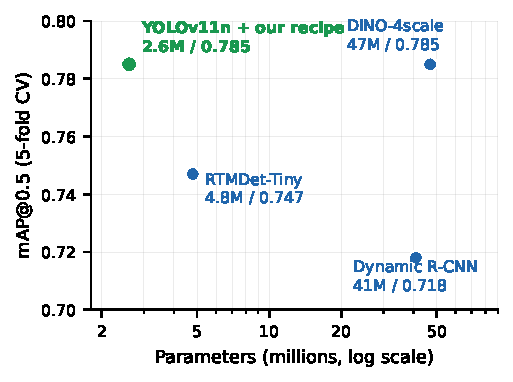
\includegraphics[width=\columnwidth]{figures/fig_frontier.pdf}
\caption{Accuracy versus model size under identical 5-fold cross-validation. The 2.6M-parameter YOLOv11n with the proposed data-centric recipe ties the 47M-parameter DINO-4scale on \map{}; the MMDetection baselines run at default training configurations, and parameters are the only efficiency axis collected.}
\label{fig:frontier}
\end{figure}

\subsection{External data: a systematic negative result}
\label{sec:external}
Table~\ref{tab:external} summarizes the exploratory campaign on the fixed split (seed-averaged; baseline \dd{} AP $0.641\pm0.036$ over 11 seeds); its rows share one protocol and report per-condition run counts, with ladder conditions reported as the range across doses. Every external-data route failed to beat the baseline on the rare class: direct mixing at any dose (0.58--0.65 across ratios 1:1 to 11.7:1, $n{=}8$) and scale-matched curation (0.63--0.65, $n{=}3$, with recall dropping to 0.51). Two further routes are reported in text rather than tabulated because their logging is heterogeneous: pretrain-then-finetune schedules, none of whose runs improved on the baseline (their run-log group is pooled with two architecture ablations, combined range 0.59--0.69, and cannot be cleanly disaggregated); and in-domain source pretraining on the 10{,}698-image inspection pool, evaluated under the clean-benchmark protocol of Section~\ref{sec:decon}, which was outright negative transfer, $-7.5$ \map{} points versus COCO initialization. Two controls localize the failure: a model trained and evaluated \emph{within} the external distribution reaches ${\approx}0.91$ \dd{} AP---the external labels are learnable---and the clean bird-nest addition lifted its own target class by $+0.136$ (0.762$\to$0.898). External data fails here not because it is unlearnable but because its notion of ``defective'' and its capture distribution do not match the target's; the signature is a recall drop at held precision. Even the healthy control carries a cost: single-class external images leave co-occurring components unlabeled, degrading Broken Insulator by $-0.12$---partial annotation is a real tax on any single-class harvest. Meanwhile the entirely native champ recipe reached $0.699\pm0.027$ on the same split. Combined with the contamination audit (Section~\ref{sec:leakage}), the practical guidance is blunt: for rare-defect classes, exhaust native data-centric levers before harvesting, and never harvest without a leakage gate.

\begin{table}[t]
\caption{External-data routes vs.\ the native recipe: fixed split, one protocol, seed-averaged \dd{} AP. $n$ = runs; ladder rows report the range across doses. Baseline $0.641\pm0.036$ (11 seeds). Pretrain-then-finetune and in-domain source pretraining are reported in the text (heterogeneous logging or different protocol).}
\label{tab:external}
\centering
\footnotesize
\setlength{\tabcolsep}{4pt}
\begin{tabular}{lcc}
\toprule
Condition & $n$ & DD AP \\
\midrule
mixing, 1:1--11.7:1 dose ladder & 8 & 0.58--0.65 \\
scale-matched mixing & 3 & 0.63--0.65 \\
\midrule
in-distribution control (external test) & 4 & ${\approx}0.91$ \\
clean bird-nest add (target class) & 1 & Birdnest $+0.136$ \\
\midrule
native champ recipe (ours) & 11 & $\mathbf{0.699\pm0.027}$ \\
\bottomrule
\end{tabular}
\end{table}

\subsection{Ablations: what moves the rare class, and what does not}
\label{sec:ablate}
\textbf{Recipe components (fixed split).} Removing only the scale-down augmentation leaves \dd{} AP within noise ($0.709$, 2 seeds) but costs 2.3 \map{} points ($0.724$ vs.\ $0.747$); high resolution alone fixed Normal Damper (${\to}0.84$) but not the defective class; oversampling with scale-aug at 640\,px reaches only $0.661\pm0.058$. Each lever alone falls short on at least one metric; the full combination delivers the seed-verified $+0.058$ \dd{} gain and the \map{} gain together. The scale-jitter sweet spot is 0.85--0.9; weaker and stronger both regress. Oversampling $\times6$ helps only at high resolution ($0.751$ at 1280\,px vs.\ $0.635$ at 640\,px, where it overfits the duplicated minority); similarly, extending stage one to 300 epochs does not help (DD $0.646$, \map{} $0.686$). \textbf{Freezing hurts.} Freezing 10 backbone layers costs $-5$ \map{} points ($0.696$); freezing 20 collapses training ($0.448$)---consistent with \cite{tsai2025atli} and opposite to classification-side practice \cite{shakiba2022insulator}. \textbf{Architecture patches underperform data levers.} A P2 high-resolution detection head improved the dominant damper class but not the defective one; copy-paste augmentation \emph{hurt} the defective class (paste artifacts); test-time augmentation was worthless ($+0.002$, rejected).

\textbf{Augmentation ablation at 768\,px (clean benchmark, 3 seeds/arm, 30 runs).} The only arm that improved on the deployment recipe was extending mosaic-free final epochs (\texttt{close\_mosaic} 20): $0.767\pm0.003$ \map{}, \dd{} $0.708\pm0.051$. Rotation is actively harmful for axis-aligned detection: $10^{\circ}$ costs $-0.10$ \dd{} AP and $45^{\circ}$ costs $-0.037$ \map{} via axis-aligned box inflation, an effect absent from the literature, where rotation is standard practice \cite{bao2022bcyolo,maduako2022felect,sadykova2020inyolo}. Disabling mosaic costs $-0.030$ \map{}; removing oversampling costs $-0.07$ \dd{} AP (rotation is not a substitute for it); oversampling all defect classes at 768\,px trades \dd{} AP ($0.567$) for Self-Exploded AP ($0.875$). Robustness is a caveat for the whole family: eval-time motion blur of 7\,px drops \map{} by $0.246$ (and Gaussian $\sigma{=}2$ to $0.442$), so blur-augmented training is required future work before flight deployment.

\begin{figure*}[t]
\centering
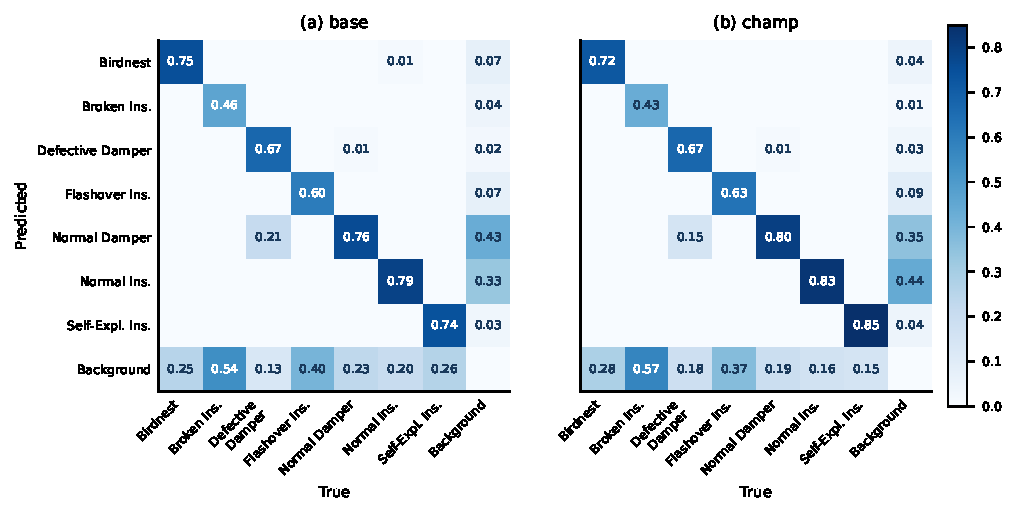
\includegraphics[width=0.88\textwidth]{figures/fig_cm.pdf}
\caption{Illustrative error structure: column-normalized confusion matrices (single fixed-split runs, confidence 0.25; re-rendered from the archived run artifacts). By the protocol argument of Section~\ref{sec:protocol}, cell-level values carry single-draw noise and are read qualitatively. In this draw, the champ recipe reduces the two flagged damper failure modes---defective dampers predicted as Normal Damper ($0.21{\to}0.15$) and spurious Normal Damper detections ($0.43{\to}0.35$)---and raises the detected fraction of the flashover, normal, and self-exploded insulator classes (Self-Exploded $0.74{\to}0.85$, misses $0.26{\to}0.15$); Broken Insulator is flat to slightly down ($0.46{\to}0.43$) in this single draw. The remaining regression is Normal Insulators false positives ($0.33{\to}0.44$).}
\label{fig:cm}
\end{figure*}

\textbf{Error structure.} Fig.~\ref{fig:cm} is one fixed-split run per condition and---by our own protocol argument (Section~\ref{sec:protocol})---is read qualitatively, not cell-by-cell; seed- or fold-aggregated matrices are outstanding analysis. With that caveat, the single-draw gains land where the recipe aims: defective-as-normal damper confusion drops ($0.21{\to}0.15$), spurious Normal Damper detections drop ($0.43{\to}0.35$), and Self-Exploded misses fall $0.26{\to}0.15$. One observation is structural and holds in both matrices: insulator defects are essentially never mislabeled \emph{as} normal insulators---their failure mode is missed detection, consistent with the recall-driven seed-averaged picture (Table~\ref{tab:cv}). We therefore \emph{conjecture} that detect-then-classify architectures \cite{zhang2023padetr,souza2023hybridyolo} address a confusion this dataset mostly does not have, while the miss-driven failure it does have responds to resolution and sampling.

\subsection{Oriented bounding boxes}
\label{sec:obb}
Under OBB training, osall v11n is the best condition (\map{} $0.817\pm0.017$) and gains shift toward Broken Insulator ($+0.10$--$0.16$) and defect recall; notably the \emph{baseline} has the best OBB \dd{} AP ($0.798\pm0.024$)---dampers are compact, so high-resolution oversampling adds little once boxes rotate. A detection-run-on-identical-folds control shows task mode is a wash overall (0.802 vs.\ 0.808 \map{}), with OBB's real benefit being box tightness on elongated classes (38\% area reduction on Normal Insulators). One OBB configuration deserves note as a maximum-recall operating point: in the 768\,px clean-benchmark ablation (single split, not these CV folds), OBB with $45^{\circ}$ rotation augmentation reaches \dd{} \emph{recall} 0.957 (AP 0.738)---rotation helps precisely where boxes can rotate with the object, inverting its axis-aligned harm. OBB labels came from a separate annotation export, so OBB and detection absolute values are not directly comparable; all OBB comparisons here are within-task.

\subsection{Decontamination: which conclusions survive clean data}
\label{sec:decon}
Removing all 249 CPLID-duplicate images from the 1{,}046-image extended target set (and re-tightening insulator boxes) yields a 797-image clean benchmark (561/116/120). On it, the recipe's headline margin survives essentially unchanged: baseline $0.736\pm0.015$ vs.\ champ $\mathbf{0.784\pm0.011}$ \map{} (3 seeds; Fig.~\ref{fig:perclass}), with the largest per-class gain on Self-Exploded Insulator ($+0.116$). The clean test split, however, contains only 12 \dd{} instances, so its \dd{} numbers ($0.614\to0.622$) are directional only---a direct illustration of why rare-class evaluation needs pooled protocols (Section~\ref{sec:protocol}). Contamination touched specific classes: every removed image carried a Self-Exploded Insulator (249 instances) plus 277 Normal Dampers, and clean-benchmark Self-Exploded AP is nominally lower (champ $0.883{\to}0.871$; protocols and test sets differ, so we read this as directional only). Finally, as a labeled ablation outside the declared primary configurations (Section~\ref{sec:protocol}), restoring the 249 CPLID images to \emph{training only} (test kept clean) sets the numerically best clean-test result at 1280\,px ($0.802\pm0.015$ \map{}, Self-Exploded $0.907$)---yet the same restore \emph{hurts} the 768\,px deployment retrain ($0.747$ vs.\ $0.766$). We conjecture a resolution-dependent interaction---at 1280\,px the added Self-Exploded instances outweigh the CPLID domain shift, at 768\,px they do not---and testing it is future work. Because adopting the restore only where it helps would be post-hoc selection, no headline or deployment number uses the restored variant; we report it as evidence that clean \emph{evaluation} does not require discarding the duplicates' training value. Contaminated-vs-clean is thus not a scandal but a measurement: the recipe's conclusions replicate, while class-level absolute numbers shift in explainable directions.

\begin{figure*}[t]
\centering
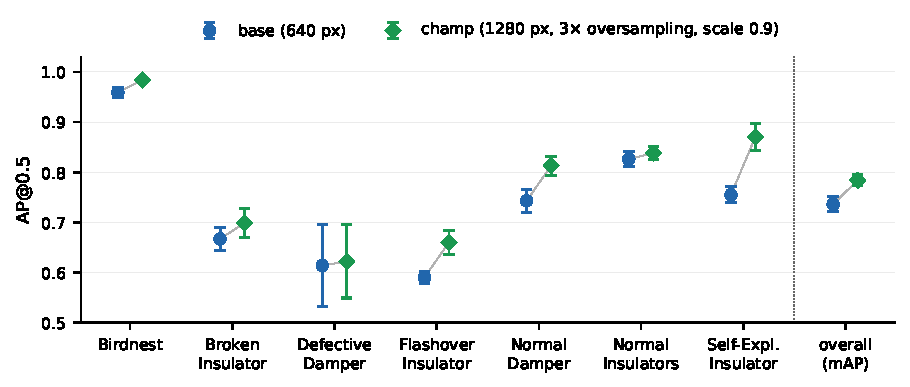
\includegraphics[width=\textwidth]{figures/fig_perclass_clean.pdf}
\caption{Per-class AP@0.5 on the decontaminated benchmark (797 images; 120-image test; 3 seeds, error bars = std). The recipe improves every class; the \dd{} column is directional only (12 test instances). Self-Exploded Insulator shows the largest gain ($+0.116$).}
\label{fig:perclass}
\end{figure*}

\subsection{Edge deployment}
\label{sec:edge}
Table~\ref{tab:edge} and Fig.~\ref{fig:deploy} give the resolution ladder on the clean benchmark. Inference-time downscaling of the 1280-trained model degrades gracefully, but \emph{retraining natively at 768\,px} is the better deployment point: $0.766\pm0.009$ \map{} with \dd{} AP $0.664\pm0.042$ (4 seeds)---the 768\,px retrain's \dd{} AP nominally exceeds the 1280\,px champ model's on this split, because at 12 test instances a single flaky instance dominates; the honest reading is parity within noise at 2.8$\times$ less inference compute. The deployment gate is accordingly \map{}-based: the retrain clears the \map{} floor ($\geq0.745$) with seed margin, while the \dd{} floor ($\geq0.59$) can be checked only directionally on 12 instances and remains \emph{provisional} pending an enlarged test pool or a CV-protocol validation of the 768\,px recipe, which we have not yet run. The TensorRT FP16 export costs $-0.009$ \map{} (engine $0.768$, \dd{} $0.732$ vs.\ PyTorch $0.777$/$0.725$) in an 8.1\,MB engine with ${\sim}0.6$--$0.8$\,GB CUDA context, inside the 2\,GB memory budget we set to cover the smallest Nano variant. Throughput is the unmeasured half of the story: every fps value in Table~\ref{tab:edge} is a \emph{projection} from a published 19-fps YOLOv8n TensorRT anchor on the same device, GFLOPs-scaled across a different architecture and resolution (${\pm}20$--$30\%$); end-to-end latency, peak memory, and power draw on the device have not been measured, and no throughput number here should be read as verified---measurement with the compiled engine is the immediate next step. Against the project's original 30\,fps real-time target, the projected ${\sim}18$\,fps at 768\,px falls short; a separate coverage memo argues that line-following still-image inspection needs only 5--10\,Hz (${\sim}26$ sightings per component per pass at 5\,Hz), but its flight-profile parameters (speed, altitude, field of view) are not reproduced here, and faster flight or video-based tracking would restore the higher requirement. Full-1280 real-time would require a modern module (e.g., Orin Nano). INT8 is unavailable on Maxwell, and pruning with a gentle-LR recovery schedule missed badly ($1.5\times$ prune: $0.609$ \map{}; a higher-LR recovery schedule remains under evaluation), so FP16 is the export format. Consistent with \cite{vazquez2026wildfire}, all accuracy-side interventions in this paper are free at inference: the recipe changes what the engine \emph{learned}, not its speed.

\begin{table}[t]
\caption{Deployment ladder on the clean benchmark (YOLOv11n; champ recipe except the 640\,px baseline row). All fps values are \emph{projections} for an original Jetson Nano from a 19-fps YOLOv8n TensorRT anchor ($\pm$20--30\%); none is measured. Bold: selected deployment configuration (\map{} gate; the \dd{} floor is provisional at 12 test instances).}
\label{tab:edge}
\centering
\footnotesize
\setlength{\tabcolsep}{4.5pt}
\begin{tabular}{lccc}
\toprule
Configuration & \map{} & DD AP & proj.\ fps \\
\midrule
640 native baseline & 0.736 & 0.614 & ${\sim}25$ \\
768 infer (1280-trained) & 0.754 & 0.593 & ${\sim}18$ \\
\textbf{768 native retrain} & $\mathbf{0.766\pm0.009}$ & $\mathbf{0.664\pm0.042}$ & ${\sim}18$ \\
1024 infer (1280-trained) & 0.783 & 0.634 & ${\sim}10$ \\
1280 native champ & 0.784 & 0.622 & ${\sim}6$ \\
\midrule
TRT FP16 engine @768 & 0.768 & 0.732 & ${\sim}18$ \\
\bottomrule
\end{tabular}
\end{table}

\begin{figure}[t]
\centering
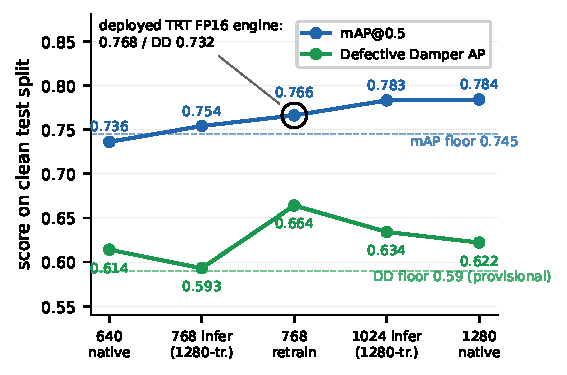
\includegraphics[width=\columnwidth]{figures/fig_deploy.pdf}
\caption{Accuracy versus input size with \emph{projected} (unmeasured) Jetson Nano throughput (per-configuration fps in Table~\ref{tab:edge}). The 768\,px native retrain (circled) clears the \map{} floor (dashed, $\geq 0.745$) with seed margin; the \dd{} floor (dashed, $\geq 0.59$) is provisional given the 12-instance test pool. The deployed TensorRT FP16 engine loses 0.009 \map{} relative to PyTorch.}
\label{fig:deploy}
\end{figure}

\section{Discussion}
\label{sec:discussion}
\textbf{What transfers is consistency, not proximity.} Our results and the literature disagree on external data only superficially. FASDD-to-wildfire transfer succeeded with a large \emph{curated} source sharing the target's label semantics \cite{vazquez2026wildfire}; our damper harvests failed with sources whose notion of ``defective'' differs from the target's, and our in-domain pool---45.3\% tower/line boxes from a single capture campaign, with two target classes absent---produced negative transfer despite being nominally on-domain. The in-distribution control (${\approx}0.91$) pins the failure on the source-target relationship, not the source. We conjecture the operative variable is \emph{label-style and curation consistency}: a source only helps when its annotation semantics and object statistics match the target's, which domain proximity does not guarantee.

\textbf{Evaluation practice is a bigger lever than architecture.} Three findings here---the $0.22$ fold-to-fold swing in rare-class AP, the 3--6 point single-split pessimism affecting even 47M-parameter baselines, and public-set duplication into the evaluation split---would each be invisible in the field's dominant single-split protocol. We suspect some published gains on small inspection benchmarks are re-drawings of split luck or contamination, and we would encourage rare-class claims to come with repeated-split means and a provenance audit; ours is, to our knowledge, the first leakage audit reported for this benchmark family.

\textbf{Dampers remain the hard class, for identifiable reasons.} Our cross-validated \dd{} AP of 0.812 sits at the favorable end of published damper-defect results (AP@0.5 0.40--0.64 in \cite{su2024cessd,zhang2024dsanet}; AP$_{75}$ 0.371 in \cite{zhang2024hcvit}), using no damper-specific architecture. The error analysis (single-run, read qualitatively; Section~\ref{sec:ablate}) suggests why the gap persists: the residual failure appears to be missing small, rare objects---not confusing them with normal ones---which caps what classification-side fixes can add and keeps resolution, sampling, and (per \cite{vieiraesilva2021stnplad}) native image resolution as the binding constraints.

\textbf{Limitations.} (i)~The clean-split \dd{} test pool (12 instances) supports only directional per-class claims; growing the defective-damper test pool is the single highest-value data investment, and the deployment recipe's \dd{} floor is unverified until then. (ii)~Jetson throughput is projected, not measured: on-device latency, peak memory, and power draw are outstanding, so every deployment claim is export-level only. (iii)~Training cost is reported structurally, not in hours (per-condition wall-clock was not logged, unlike \cite{tsai2025atli}), and FLOPs/latency for the MMDetection baselines were not collected, leaving parameters as the only---imperfect---efficiency proxy in Table~\ref{tab:sota}. (iv)~The heavyweight baselines are untuned: the data-centric levers are model-agnostic in principle and might lift DINO or RTMDet as well; until a matched-budget tuned-heavyweight control is run, our claim is limited to stock baselines. (v)~ATLI's imagery skews toward one grid's infrastructure (18.5\% was CPLID-derived); geographic generalization is untested. (vi)~Blur fragility ($-0.246$ \map{} at 7\,px motion blur) must be addressed before real flight video. (vii)~OBB comparisons are within-task only, due to a separate annotation export.

\section{Conclusion}
On a small, imbalanced transmission-line defect benchmark, we showed that the rare-class bottleneck yields to data-centric treatment of the \emph{native} dataset---high-resolution training, minority oversampling, and scale-down augmentation---validated by proper cross-validation, where the 2.6M-parameter model ties a 47M-parameter transformer on \map{} and is comparable on the rare class. External data harvesting failed at every dose and schedule despite learnable labels; provenance auditing exposed evaluation-set contamination from three public sources; and the recipe survived decontamination and exported to an FP16 engine sized for a Jetson Nano, with on-device throughput, memory, and power measurement the outstanding step before any deployment claim is final. Future work: measured on-device benchmarking (and Orin-class hardware for full-resolution real time), matched-budget application of the data-centric levers to a heavyweight baseline, per-condition training-cost accounting, class-weighted/focal losses for the normal-versus-defective split (untried field-wide), detect-then-classify heads for the residual confusion, blur-robust training, and enlarging the defective-damper evaluation pool, which currently limits per-class certainty more than any modeling choice.

\bibliographystyle{IEEEtran}
\bibliography{refs,refs_extra}

\end{document}
